\chapter{Ανίχνευση αντικειμένων}\label{ch:facedetection}

Στο κεφάλαιο αυτό γίνεται μια παρουσίαση του αλγορίθμου των Viola-Jones για την
ανίχνευση αντικειμένων. Παρόλο που ο αλγόριθμος της μεθόδου μπορεί να εκπαιδευτεί
και να αναγνωρίσει κάθε είδους αντικέιμενα, χρησιμοποιείται περισσότερο στην
αναγνώρηση προσώπων. Εδώ, θα αναλύσουμε την τεχνική feature extractions πάνω στην
οποία βασίζεται αυτή μέθοδος για τα πρόσωπα. Στο τέλος ο αναγνώστης θα πρέπει
να έχει κατανοήσει τα διάφορα στάδια του αλγορίθμου και την αρχή λειτουργίας
της μεθόδου.

\section{Συνοπτική παρουσίαση μεθόδων ανίχνευσης κλάσεων αντικειμένων}\label{sec:facedetmethods}

In recent years, virtualization has become an important consideration and has
gained popularity in many different areas such as server consolidation, cloud
computing, corporate data centers, and the academic world. This is largely due
to an increase in hardware performance of about ten fold in the past decade, the
need to reduce the capital and operational cost to the minimum~\cite{Graziano},
and the desire to run multiple operating systems in a single host.

\begin{flushright}
  \emph{``A virtual machine is taken to be an efficient,\\
        isolated duplicate of the real
        machine."}~\cite{DBLP:journals/cacm/PopekG74}


  Gerald J. Popek and Robert P. Goldberg
\end{flushright}
The definition of virtual machine has evolved since then, and current virtual
machine uses have not direct correspondence to any real hardware, necessarily,
and are used in a number of subdisciplines ranging from operating systems to
programming languages to processor architectures~\cite{smith_nair}. Depending on
the correspondence degree of a physical machine, virtual machines can be
classified into two major categories. The \emph{Process Virtual Machines} and
the \emph{System Virtual Machines}.


\subsection{Η μέθοδος PCA (Principal Components Analysis)}

\emph{Type I} hypervisors, also called native or ``bare metal" ones, run
directly on the physical hardware, control it, and manage the guest operating
systems that run on a different level above the hardware, as Figure
\ref{fig:hypervisors} denotes. They are completely independent from the
operating system, and are also responsible for many basic operations like VM
scheduling, memory management, and more. They allow
multiple commodity operating systems run concurrently and share conventional
hardware in a safe way, but without sacrificing either performance or
functionality. Most known hypervisors of that type are the \emph{VMWare vShpere
Hypervisor}~\flink{http://www.vmware.com/products/vshpere-hypervisor/} and the
\emph{Xen Hypervisor}~\cite{xen_art}.

\begin{figure}[htbp]
  \begin{center}
    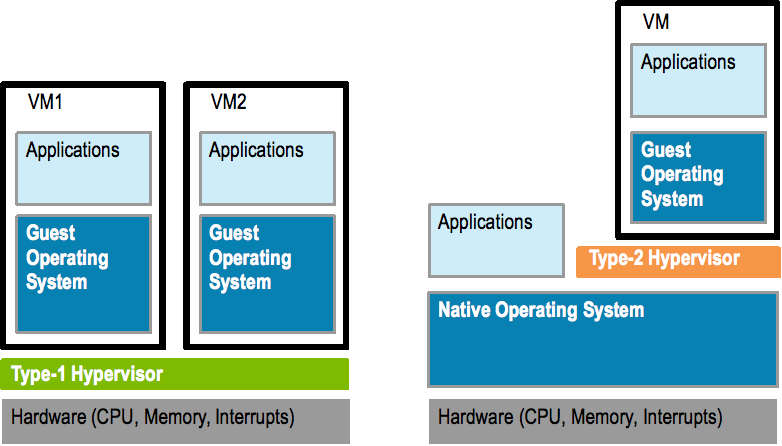
\includegraphics[width=0.8\maxwidth]{../figures/type1-vs-2.png}
    \caption{Hypervisor types\label{fig:hypervisors}}
   \end{center}
\end{figure}


\subsection{H μέθοδος Edge Orientation}

Full Virtualization is a hardware virtualization type on which the virtual
machine simulates almost completely the actual hardware to allow the guest
operating system software, mainly, to be run transparently and in isolation from
the rest system. That implies that every single feature of the physical hardware
can be reflected into a virtual machine, including interrupts, memory access,
and whatever other elements are used by the software that runs on the bare
machine.


\subsection{H μέθοδος Hausdorff Distance}

This technique does not simulates a hardware environment. However, the guest
applications are executed in their own isolated domains, as if they are running
on a separate system. With Paravirtualization the term of \emph{hypercall} is
introduced. The guest para-virtualized operating systems should make a system
call to the underlying hypervisor when it have to perform a privileged
operation. By allowing the guest OS to indicate its intents to the hypervisor,
improved performance and efficiency can be achieved, as each OS can cooperate to
obtain better performance when running in a virtual machine. As a result, the
guest OS have to be modified for the hypervisor, since the virtualization code
is integrated into the operating system itself. \emph{Xen} and \emph{User Mode
Linux} are examples of paravirtualization solutions.

\section{H μέθοδος Viola-Jones}\label{sec:violjon}

O αλγόριθμος των Viola-Jones~\cite{Viola01rapidobject} υπήρξε τομή στο πεδίο
της ανίχνευσης αντικειμένων σε εικόνες. Ουσιαστικά δημιούργησε την πρώτη
υποδομή ανίχνευσης αντικειμένων η οποία παρήγαγε ανταγωνιστικά αποτελέσμα σε
πραγματικό χρόνο. Παρόλο που σχεδιάστηκε ώστε να μπορεί να εκπαιδευτεί με σκοπό
να αναγνωρίζει οποιαδήποτε κλάση αντικειμένων, ουσιαστικά ο αρχικός σχεδιασμός
του αλγορίθμου έγινε με γνόμωνα την αναγνώρηση προσώπων σε εικόνες. Εν τέλει
εκεί εντοπίζεται και το μεγαλύτερο ποσοστό της χρήσης του.

Τα βασικά χαρακτηριστικά του ανωτέρο αλγορίθμου είναι:
\begin{description}
  \item[Αξιοπιστία] \hfill \\
      Ο αλγόριθμος έχει πάντα υψηλό ποσοστό σωστών ανιχνεύσεων (true-positives)
        και χαμηλό ποσοστό λάθος ανιχνεύσεων (false-ositives)
  \item[Ταχύτητα πραγματικού χρόνου] \hfill \\
      Σε εφαρμογές πραγματικού περιβάλλοντος επεξεργάζονται τουλάχιστον 2 εικόνες
        (frames) ανά δευτερόλεπτο
  \item[Αναγνώρηση προσώπων] \hfill \\
      Ο αλγόριθμος έχει στόχο να ανιχνέυει πρόσωπα από μη-πρόσωπα. Δεν έχει
        σκοπό να αναγνωρίζει τα πρόσωπα που ανιχνεύει
\end{description}

Για να το πετύχει αυτό ο αλγόριθμος χρησιμοποιεί κατά σειρά τα παρακάτω στάδια
τα οποία θα αναλύσουμε εκτενέστερα στη συνέχεια:
\begin{itemize}
 \item Επιλογή χαρακτηρισικών τύπου Haar (Haar features selection)
 \item Κατασκευή ολοκληρώματος εικόνας (Integral image creation)
 \item Εκπαίδευση του αλγορίθμου AdaBoost (AdaBoost training)
 \item Χρήση ενός διαδοχικά διασυνδεδεμένου ταξινομητή (Cascade classifier)
\end{itemize}

\subsection{Χαρακτηριστικά τύπου Haar}

Για να ανιχνεύσουμε αντικείμενα σε εικόνες απαιτείται κατάλληλη επεξεργασία και
αναπαράσταση του περιεχομένου τους. Για την αναπαράσταση του περιεχομένου της εικόνας στη
μέθοδο που εξετάζουμε, χρησιμοποιούμε τα χαρακτηριστικά τύπου Haar, τα οποία προκύπτουν
από την εφαρμογή του μετασχηματισμού κυματιδίων σε μια εικόνα με χρήση των συναρτήσεων
τύπου Haar~\cite{Viola01rapidobject}.

Η χρησιμοποίηση των συναρτήσεων Haar στο μετασχηματισμό κυματιδίων ξεκινά από την
παρατήρηση ότι η τιμή της φωτεινότητας κάθε εικονοστοιχείου επηρεάζεται έντονα από τις
        αλλαγές στο φωτισμό της σκηνής~\cite{OrePapSinOsu97}. Αυτή η αλλαγή όμως, επηρεάζει αρκετά ομοιόμορφα
όλα τα εικονοστοιχεία της εικόνας. Έτσι, η τιμή μιας συνάρτησης που εξετάζει τη μέση διαφορά
ανάμεσα σε δύο ή τρεις περιοχές της ίδιας εικόνας, θα παραμένει σε μεγάλο βαθμό ανεπηρέαστη.
Χρησιμοποιώντας, λοιπόν, τις συναρτήσεις Haar, η διαδικασία της ανίχνευσης αντικειμένων δε θα
επηρεάζεται από τις διαφορές στη φωτεινότητα από εικόνα σε εικόνα.

Οι συναρτήσεις Haar υπολογίζουν τη διαφορά ανάμεσα στους μέσους όρους των τιμών των
εικονοστοιχείων δύο (ή τριών) περιοχών. Ας θεωρήσουμε τη συνάρτηση Haar που παριστάνεται με
το ορθογώνιο i από το Σχήμα 2.1. Υπολογίζεται ο μέσος όρος των εικονοστοιχείων που
βρίσκονται μέσα στο άσπρο ορθογώνιο, καθώς και αυτών που βρίσκονται μέσα στο μαύρο
ορθογώνιο. Έπειτα, ο μέσος όρος του μαύρου ορθογωνίου αφαιρείται από τον μέσο όρο του
άσπρου. Η τιμή που προκύπτει αποτελεί την τιμή του Haar χαρακτηριστικού.

Εφαρμόζοντας τον μετασχηματισμό κυματιδίων με τη συναρτησιακή βάση Haar, προκύπτει
ένας περιορισμένος αριθμός χαρακτηριστικών~\cite{OrePapSinOsu97}. Στο μονοδιάστατο μετασχηματισμό, η
απόσταση ανάμεσα σε δύο γειτονικά κυματίδια, σε επίπεδο n , θα είναι 2 n . Η απόσταση αυτή είναι
πολύ μεγάλη, κι έτσι δεν λαμβάνουμε όσες πληροφορίες θέλουμε από μια εικόνα ώστε να την
- 21 -περιγράψουμε λεπτομερώς. Για να έχουμε, λοιπόν, μια πιο λεπτομερή, χωρικά, αναπαράσταση του
περιεχομένου της εικόνας χρειαζόμαστε ένα σύνολο από πλεονάζουσες συναρτήσεις βάσης. Για να
το πετύχουμε αυτό, εφαρμόζουμε τις συναρτήσεις Haar με μεταξύ τους απόσταση ένα
εικονοστοιχείο κάθε φορά. Έτσι, θα έχουμε μια πολύ πιο πυκνή αναπαράσταση. Επίσης, στο
μετασχηματισμό κυματιδίων, το μέγεθος των συναρτήσεων Haar, κανονικά διπλασιάζεται σε κάθε
επανάληψη. Για να αυξήσουμε ακόμα περισσότερο την λαμβανόμενη πληροφορία από την εικόνα,
ορίζουμε ότι το μέγεθος των συναρτήσεων Haar θα αυξάνει κάθε φορά κατά ένα μόνο
εικονοστοιχείο. Έτσι, το σύνολο των χαρακτηριστικών Haar σε μία εικόνα γίνεται
υπερπολλαπλάσιο του αρχικού. Αυξάνουμε, δηλαδή, την ποσότητα της πληροφορίας που αντλούμε
από μια εικόνα, αυξάνοντας τα χαρακτηριστικά τύπου Haar που θα υπολογιστούν σε αυτήν.

Τα κλασσικά Haar χαρακτηριστικά φαίνονται στο Σχήμα 2.1α ~\cite{OrePapSinOsu97}. Είναι σχετικά απλά
και μπορούν να εντοπίσουν ακμές οριζόντια και κατακόρυφα καθώς και διαγώνιες γραμμές. Για να
μπορέσουμε να αναπαραστήσουμε γραμμές, ράβδους και τετράγωνα καλύτερα, προσθέτουμε τα
χαρακτηριστικά που φαίνονται στο Σχήμα 2.1β (τα χαρακτηριστικά iv και v εμφανίζονται στο
~\cite{Viola01rapidobject}, ενώ τα υπόλοιπα στο ~\cite{Lienhart02anextended},
τα οποία υπολογίζονται χωρίς να αυξάνεται ιδιαίτερα η
πολυπλοκότητα, όπως θα δούμε στην ενότητα 2.2. Μια μεγάλη προσθήκη είναι τα χαρακτηριστικά
που είναι περιστραμμένα κατά 45 0 και φαίνονται στο Σχήμα 2.1γ ~\cite{Lienhart02anextended}. Με τη χρήση αυτών
βελτιώνεται σημαντικά η αναπαράσταση των διαγώνιων σχημάτων. Με την προσθήκη όλων αυτών
των χαρακτηριστικών, το σύνολο γίνεται υπερπλήρες και αναπαριστά πολύ καλύτερα την
πληροφορία που περιέχεται σε μία εικόνα.

Although the Cloud Computing became known to the public the last decade, that
does not constitutes a new invention or a revolution for the computer science.
It is more an evolution of already existing technologies rather than a new
computing paradigm. The following short historical review of the development of
computers and the Internet will show us that the idea of a centralized computer
utility was always existed and inevitably lead us to the beginning of Cloud
Computing~\cite{cloud_evolution}.


\begin{figure}[htbp]
  \begin{center}
    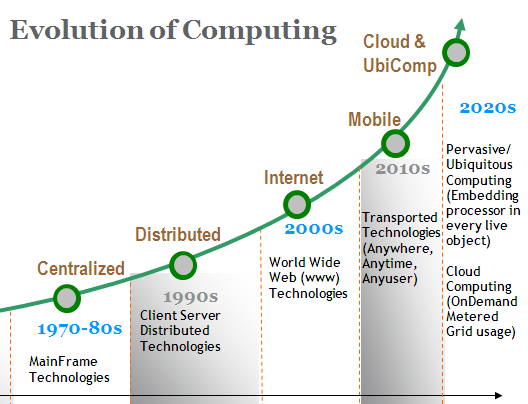
\includegraphics[width=0.75\maxwidth]{../figures/comp_evol.png}
    \caption{Computer history timeline\label{fig:comp_evol}}
   \end{center}
\end{figure}

Για τον υπολογισμό του πλήθους των Haar χαρακτηριστικών σε κάποιο παράθυρο εικόνας
πλάτους W και ύψους H, ακολουθούμε την παρακάτω διαδικασία [LiMa02]. Έστω ότι w και h
είναι το πλάτος και ύψος του ορθογωνίου της συνάρτησης Haar που εξετάζουμε. Το μέγεθος του
ορθογωνίου θα αυξάνεται κατά ένα σε κάθε βήμα. Άρα, οι μέγιστοι συντελεστές μεγέθυνσης των
 W 
 H 
ορθογωνίων σε πλάτος και ύψος θα είναι X =   και Y =   , αντίστοιχα. Το πλήθος των
 w 
 h 
χαρακτηριστικών που προκύπτουν από την εφαρμογή ενός κατακόρυφου Haar χαρακτηριστικού
στο παράθυρο εικόνας, είναι:


\begin{table}[htbp]
  \centering
  \begin{tabular}{ | l | l | }
    \hline
    Component & Description \\ \hline \hline
    CPU & 8 x QEMU Virtual CPU Version 1.7.0 \\
    \hline
    RAΜ & 8192 MB  \\
    \hline
    Disk & 80 GB \\
    \hline
  \end{tabular}
  \caption{Test-VM hardware specs}
  \label{tab:hw-specs}
\end{table}


\subsection{Ολοκλήρωμα εικόνας}

Cloud computing services can be classified along different layers, according to
the level of the capability they provide. There are three primary models, as
shown in Figure~\ref{fig:cloud_layers}, namely: Infrastructure as a Service
(\emph{IaaS}), Platform as a Service (\emph{PaaS}), and Software as a Service
(\emph{SaaS}). These abstraction levels can also be viewed as a layered
architecture where services of higher levels can be composed from the underlying
layers.

\begin{figure}[htbp]
  \begin{center}
    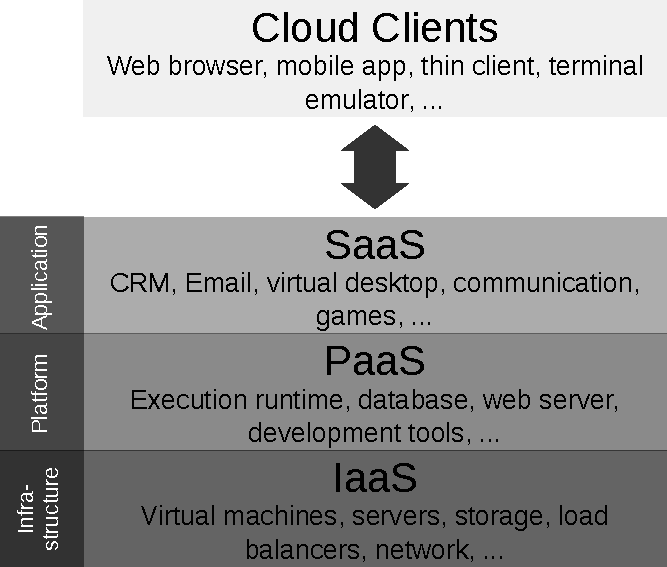
\includegraphics[width=1.0\maxwidth]{../figures/cloud_layers-black.pdf}
    \caption{The layers of Cloud Computing\label{fig:cloud_layers}}
   \end{center}
\end{figure}


\subsection{Ο αλγόριθμος AdaBoost}

Υπάρχουν πολλές μέθοδοι για την υλοποίηση ενός ταξινομητή, δεδομένου ενός συνόλου
χαρακτηριστικών και ενός συνόλου εκμάθησης θετικών και αρνητικών εικόνων. Έχουν
χρησιμοποιηθεί νευρωνικά δίκτυα, μηχανές διανυσμάτων υποστήριξης κ.α. Όπως είδαμε
προηγουμένως, τα χαρακτηριστικά που χρησιμοποιούμε μπορούν να υπολογιστούν πάρα πολύ
γρήγορα. Το σύνολο όμως των χαρακτηριστικών είναι πολύ μεγάλο (περίπου 120.000 για μια
εικόνα 20x20). Έτσι, ο υπολογισμός του πλήρους συνόλου των χαρακτηριστικών για την ανίχνευση
σε κάθε υποπαράθυρο της εικόνας, θα ήταν και πάλι πολύ χρονοβόρος [ViJo01]. Θα πρέπει,
λοιπόν, να επιλέξουμε ένα μικρό αριθμό χαρακτηριστικών από το διαθέσιμο σύνολο, και να
- 27 -κατασκευάσουμε από αυτά τον ταξινομητή μας. Η επιλογή αυτών των χαρακτηριστικών είναι
αρκετά δύσκολη.

Στην μέθοδο ανίχνευσης που εξετάζουμε, χρησιμοποιήθηκε ο αλγόριθμος AdaBoost τόσο για
την επιλογή των χαρακτηριστικών που θα χρησιμοποιηθούν, όσο και για την εκπαίδευση του
ταξινομητή [FrSc95]. Ο αλγόριθμος εκμάθησης AdaBoost ανήκει στην κατηγορία των
αλγορίθμων ενδυνάμωσης (boosting) και χρησιμοποιείται για να αυξήσει την απόδοση ενός
οποιουδήποτε απλού αλγορίθμου ταξινόμησης. Ο απλός αλγόριθμος ταξινόμησης λέγεται και
ασθενής αλγόριθμος ταξινόμησης, καθώς ακόμα και η καλύτερη συνάρτηση ταξινόμησης που
μπορεί να προκύψει από αυτόν, δεν αναμένεται να ταξινομεί καλά τα δεδομένα. Συγκεκριμένα,
αρκεί η συνάρτηση ταξινόμησης να έχει απόδοση ελαφρά καλύτερη από την τυχαία ταξινόμηση
(50%). Για να αυξήσει, λοιπόν, την απόδοση ενός ασθενούς αλγορίθμου ταξινόμησης, ο AdaBoost
συνδυάζει μια συλλογή ασθενών συναρτήσεων ταξινόμησης χρησιμοποιώντας άπληστο αλγόριθμο,
ώστε να σχηματίσει από αυτούς έναν ισχυρότερο ταξινομητή.

Η βελτίωση του ασθενούς αλγορίθμου ταξινόμησης πραγματοποιείται, καλώντας τον
αλγόριθμο να επιλύσει μια αλληλουχία προβλημάτων ταξινόμησης. Αρχικά, όλα τα παραδείγματα
(θετικά και αρνητικά) παίρνουν μια τιμή βάρους, η οποία είναι ίδια για όλα. ∆ίνονται στον
αλγόριθμο τα παραδείγματα και πραγματοποιείται ο πρώτος κύκλος εκμάθησης, όπου ο
αλγόριθμος ταξινομεί όλα τα παραδείγματα με κάθε διαθέσιμη συνάρτηση ταξινόμησης. Έπειτα,
οι συναρτήσεις ταξινόμησης διατάσσονται σύμφωνα με τα αποτελέσματά τους, λαμβάνοντας υπόψη
το βάρος κάθε παραδείγματος. Επιλέγεται ένας μικρός αριθμός συναρτήσεων ταξινόμησης, από
αυτές με τα καλύτερα αποτελέσματα, που αποτελούν τον πρώτο ασθενή ταξινομητή. Ο πρώτος
κύκλος εκμάθησης ολοκληρώνεται και τα βάρη των παραδειγμάτων ισοσταθμίζονται, δίνοντας
μεγαλύτερο βάρος στα παραδείγματα που ταξινομήθηκαν λανθασμένα από τον πρώτο ασθενή
ταξινομητή. Έτσι, στον δεύτερο κύκλο εκμάθησης ο αλγόριθμος ταξινόμησης θα θεωρήσει πιο
σημαντικά τα παραδείγματα που ταξινομήθηκαν λανθασμένα από τον προηγούμενο ταξινομητή.
Τα βήματα επαναλαμβάνονται διαδοχικά, μέχρι να φτάσουμε στο επίπεδο του συνολικού λόγου
λανθασμένης ταξινόμησης που επιθυμούμε. Τελικά, ο ισχυρός ταξινομητής προκύπτει από τον
συνδυασμό των ασθενών ταξινομητών που επιλέχθηκαν και ένα κατώφλι. Κατά την διαδικασία της
ταξινόμησης ενός υποπαραθύρου εικόνας από τον ισχυρό ταξινομητή, εφαρμόζονται στο
υποπαράθυρο όλοι οι ασθενείς ταξινομητές. Τα αποτελέσματα των ασθενών ταξινομητών
αθροίζονται, και αν το άθροισμα ξεπερνά το κατώφλι του ταξινομητή, το υπό εξέταση αντικείμενο
ταξινομείται ως θετικό, αλλιώς ως αρνητικό.

Υπάρχουν τέσσερις εκδοχές του αλγόριθμου AdaBoost [FrHT00]. Η αρχική εκδοχή
ονομάζεται ∆ιακριτός AdaBoost (Discrete AdaBoost – DAB) καθώς η συνάρτηση ταξινόμησης
κάθε ασθενή ταξινομητή παίρνει μόνο δύο διακριτές τιμές, τις { − 1,1  } ανάλογα με το αν ένα
δείγμα ταξινομείται ως θετικό ή αρνητικό. Η δεύτερη εκδοχή ονομάζεται Πραγματικός AdaBoost
(Real AdaBoost – RAB), καθώς η συνάρτηση ταξινόμησης κάθε ασθενή ταξινομητή παίρνει όλες
τις πραγματικές τιμές στο διάστημα [ 0,1  ] . Με τη χρήση του RAB, μπορούμε να έχουμε μια
ένδειξη εμπιστοσύνης για τα αποτελέσματα της ταξινόμησης, χρησιμοποιώντας τις τιμές που
επιστρέφονται από τον αλγόριθμο και όχι μόνο το αποτέλεσμα της θετικής ή αρνητικής
ταξινόμησης. Άλλη εκδοχή είναι ο Ήπιος AdaBoost (Gentle AdaBoost – GAB), ο οποίος
βασίζεται στον Πραγματικό AdaBoost αλλά χρησιμοποιεί βήματα της μεθόδου Newton αντί για
ακριβή υπολογισμό. Τέλος, υπάρχει και ο LogitBoost, ο οποίος έχει δύο παραλλαγές, αυτή που
χρησιμοποιεί δύο κλάσεις και αυτή που χρησιμοποιεί J κλάσεις. Ο αριθμός των κλάσεων επηρεάζει
- 28 -την τιμή της εκτίμησης πιθανότητας κάθε δείγματος x i , η οποία ισούται με p ( x i  ) =
1
στη μία
2
1
στην άλλη.
J

Στη μέθοδο ανίχνευσης αντικειμένων που χρησιμοποιούμε, κάθε ασθενής αλγόριθμος
εκμάθησης περιορίζεται στο σύνολο των συναρτήσεων ταξινόμησης που αποτελούνται από ένα
μόνο χαρακτηριστικό τύπου Haar. Προφανώς, από ένα μόνο χαρακτηριστικό δε μπορούμε να
περιμένουμε ιδιαίτερα χαμηλό λόγο σφάλματος. Σε κάθε στάδιο του αλγορίθμου AdaBoost
επιλέγεται το χαρακτηριστικό που διαχωρίζει καλύτερα τα θετικά από τα αρνητικά δείγματα. Για
κάθε χαρακτηριστικό, ο ασθενής αλγόριθμος εκμάθησης προσδιορίζει ένα κατώφλι της τιμής του
χαρακτηριστικού, που ελέγχοντάς το περιορίζονται οι λανθασμένες ταξινομήσεις από το
συγκεκριμένο χαρακτηριστικό στις ελάχιστες δυνατές. Έπειτα, επιλέγεται ως ασθενής ταξινομητής
το χαρακτηριστικό τύπου Haar, που, για το δεδομένο κατώφλι του, κάνει τη συνολικά καλύτερη
ταξινόμηση. Ο AdaBoost συνεχίζει εκπαιδεύοντας όλους τους ασθενείς ταξινομητές, μέχρι το
σημείο που ο ισχυρός συνολικός ταξινομητής επιτυγχάνει το επίπεδο ταξινόμησης που ζητάμε.
Ο αλγόριθμος AdaBoost παρέχει αρκετά ισχυρές εγγυήσεις για την ορθότητά του. Έχει
αποδειχθεί, ότι το σφάλμα ταξινόμησης του ισχυρού ταξινομητή που προκύπτει από την εφαρμογή
του αλγορίθμου, τείνει προς το μηδέν εκθετικά ως προς τον αριθμό των κύκλων εκπαίδευσης
[SFBL98]. Επίσης, η όλη διαδικασία της εκμάθησης πραγματοποιείται με μεγάλη ταχύτητα. Ας
θεωρήσουμε ότι έχουμε στη διάθεσή μας K χαρακτηριστικά τύπου Haar και
εικόνες-
παραδείγματα. Για να κατασκευαστεί ένας ισχυρός ταξινομητής από τον αλγόριθμο AdaBoost,
περίπτωση και p ( x i  ) =
που αποτελείται από M ασθενείς ταξινομητές, χρειάζονται O ( M K  ) βήματα, σε αντίθεση με
άλλους αλγορίθμους που χρειάζονται O ( M K
)
βήματα.

\subsection{Χρήση ενός Cascade Classifier}

Σε αυτή την ενότητα παρουσιάζεται η μέθοδος ταξινόμησης με χρήση ενός ∆ιαδοχικά
Συνδεδεμένου Ταξινομητή (∆ΣΤ) [ViJo01]. Η μέθοδος αυτή βοηθά στη επίτευξη υψηλού λόγου
ανίχνευσης, μειώνοντας σημαντικά τον απαιτούμενο χρόνο. Η ιδέα στηρίζεται στο γεγονός ότι
μπορούμε να κατασκευάσουμε πολλούς μικρούς σε μέγεθος ταξινομητές, τους οποίους θα
συνδέσουμε διαδοχικά. Μπορούμε, λοιπόν, να χρησιμοποιήσουμε απλούστερους και πολύ
γρήγορους ταξινομητές αρχικά, οι οποίοι θα απορρίπτουν γρήγορα την πλειονότητα των
αρνητικών υποπαραθύρων, και πιο σύνθετους και χρονοβόρους αργότερα, ώστε να μειώσουμε το
λόγο λανθασμένων ανιχνεύσεων.

Η διάταξη του ∆ΣΤ θυμίζει τη μορφή ενός εκφυλισμένου δέντρου απόφασης. Κάθε
υποπαράθυρο της εικόνας εισέρχεται στον πρώτο ταξινομητή. Αν ο ταξινομητής το κατατάξει ως
θετικό, αυτό περνά ως είσοδος στον δεύτερο ταξινομητή. Αν και αυτός το κατατάξει ως θετικό,
τότε περνά στον τρίτο κ.ο.κ. Αν σε αυτή τη διαδοχή κάποιος ταξινομητής κατατάξει το
υποπαράθυρο ως αρνητικό, τότε αυτό απορρίπτεται και δεν εξετάζεται από κανένα άλλο
ταξινομητή (βλέπε Σχήμα 2.4). Θα μπορούσαμε να παρομοιάσουμε τον ∆ΣΤ με έναν μεγάλο
ταξινομητή που αποτελείται από το σύνολο των χαρακτηριστικών του ∆ΣΤ, όπου όμως δεν
περιμένουμε να υπολογιστεί όλο το πλήθος των χαρακτηριστικών. Αντίθετα, ελέγχουμε ανά μερικά
- 29 -χαρακτηριστικά το άθροισμα των τιμών των χαρακτηριστικών για να αποφασίσουμε αν το υπό
εξέταση υποπαράθυρο απορρίπτεται ή όχι.

\begin{figure}[htbp]
  \begin{center}
    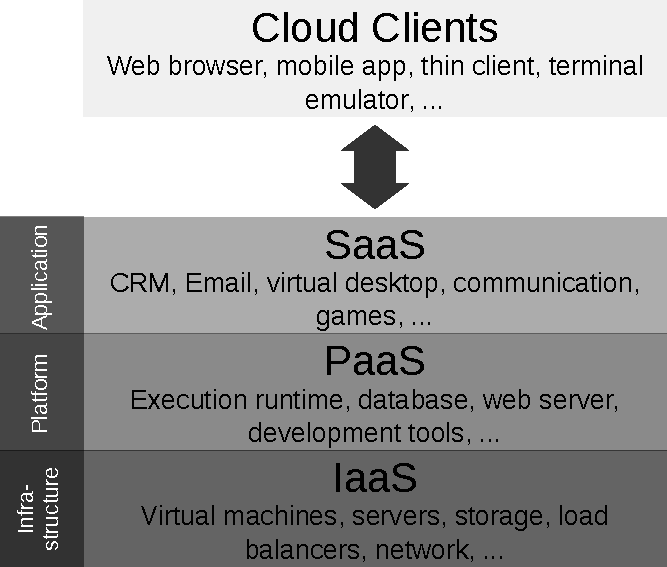
\includegraphics[width=1.0\maxwidth]{../figures/cloud_layers-black.pdf}
    \caption{The layers of Cloud Computing\label{fig:cloud_layers}}
   \end{center}
\end{figure}
\section{Άλλες μέθοδοι που έχουν χρησιμοποιηθεί}\label{sec:othermethods}

Κάθε ταξινομητής του ∆ΣΤ εκπαιδεύεται χρησιμοποιώντας ένα σύνολο θετικών και ένα
σύνολο αρνητικών παραδειγμάτων, όπως είδαμε στην ενότητα 2.3. Το σύνολο των θετικών
παραδειγμάτων είναι το ίδιο κατά την εκπαίδευση κάθε ταξινομητή. Το σύνολο των αρνητικών
παραδειγμάτων όμως, μεταβάλλεται. Συγκεκριμένα, κάθε ταξινομητής εκπαιδεύεται
χρησιμοποιώντας ως αρνητικά παραδείγματα, τα παραδείγματα που ταξινομούνται από τους
προηγούμενους ταξινομητές του ∆ΣΤ ως θετικά [ViJo01]. Αυτό αυξάνει σε πολύ μεγάλο βαθμό τα
αρνητικά παραδείγματα τα οποία θα εξεταστούν συνολικά. Για να φτάσει ένας συγκεκριμένος
αριθμός αρνητικών παραδειγμάτων στον τρέχοντα ταξινομητή, θα πρέπει τα παραδείγματα αυτά
να ταξινομηθούν από όλους τους προηγούμενους ταξινομητές του ∆ΣΤ (λανθασμένα) ως θετικά.
Ας θεωρήσουμε ότι σε κάθε στάδιο ενός ∆ΣΤ θέλουμε να εξετάζονται 1.000 αρνητικά
παραδείγματα και κάθε στάδιο έχει λόγο λανθασμένης θετικής ανίχνευσης 0,5. Τότε, για να
περάσουν στο δέκατο στάδιο 1.000 αρνητικά παραδείγματα, αυτά θα χρειαστεί να έχουν
ταξινομηθεί από τα προηγούμενα εννιά στάδια ως θετικά. Έτσι, συνολικά θα πρέπει να εξεταστούν
περίπου 512.000 αρνητικά παραδείγματα.

Η εξέταση πολύ μεγαλύτερου αριθμού αρνητικών παραδειγμάτων αυξάνει την τελική απόδοση
του ∆ΣΤ. Αντίθετα, κάθε ταξινομητής καλείται να πραγματοποιήσει μια πιο δύσκολη ταξινόμηση
από αυτές των προηγούμενων ταξινομητών. Τα αρνητικά παραδείγματα που θα έχει στη διάθεσή
του θα είναι πιο δύσκολα στην ταξινόμηση από τα παραδείγματα που είχαν τα προηγούμενα από
αυτό στάδια. Έχοντας, λοιπόν, πιο δύσκολο σύνολο εκπαίδευσης ένας ταξινομητής που βρίσκεται
σε προχωρημένο στάδιο, θα παρουσιάσει αυξημένες λανθασμένες ταξινομήσεις, θετικές και
αρνητικές.

Οι απλοί ταξινομητές ενός ∆ΣΤ, θα πρέπει να έχουν πολύ χαμηλό λόγο λανθασμένων
αρνητικών ταξινομήσεων, ώστε να μην χάνονται τα πραγματικά αντικείμενα στη συνολική
ταξινόμηση. Για να διασφαλίσουμε τη σωστή λειτουργία του ∆ΣΤ, θα πρέπει να αυξήσουμε
περαιτέρω τις θετικές ταξινομήσεις (είτε αφορούν πραγματικά αντικείμενα είτε όχι) [ViJo01]. Μια
τεχνική για να πετύχουμε αυτό το αποτέλεσμα είναι να επέμβουμε στις τιμές των κατωφλίων των
ταξινομητών που προσδιόρισε ο αλγόριθμος AdaBoost κατά την εκπαίδευση. Το κατώφλι ενός
ταξινομητή ορίζει την ελάχιστη τιμή του σταθμισμένου με βάρη αθροίσματος των τιμών των
χαρακτηριστικών που θα πρέπει να έχει ένα υποπαράθυρο για να ταξινομηθεί ως θετικό. Ένα
υποπαράθυρο ταξινομείται, δηλαδή, ως θετικό, όταν το (σταθμισμένο) άθροισμα των τιμών των
- 30 -χαρακτηριστικών που υπολογίστηκε για αυτό ξεπερνά το κατώφλι του ταξινομητή. Έτσι,
μειώνοντας τις τιμές των κατωφλίων θα αυξηθεί ο αριθμός των παραθύρων που ταξινομούνται ως
θετικά, άρα και ο λόγος θετικών ταξινομήσεων

\subsection{NoSQl compromises}

Companies want solutions that would scale, be fast, and operationally efficient.
They also ideally expect operations to speed up by simply adding new commodity
hardware, at almost a linear rate. One major bottleneck to accomplish that goal
are the database systems. So, in order to achieve the desired behavior, some
compromises should be made, and a bunch of tradeoffs should be taking into
account~\cite{burd}.

\begin{description}\label{item:cap}
  \item[The CAP Theorem] \hfill \\
    In \emph{2000}, Berkeley's CA researcher Eric Brewer published the CAP
    Theorem~\flink{http://en.wikipedia.org/wiki/CAP\_theorem}, also known as
    Brewer's Theorem. What Brewer claimed is that it is impossible for a
    distributed system to continually maintain perfect \emph{C}onsistency,
    \emph{A}vailability, and \emph{P}artition tolerance.

    \begin{itemize}
      \item \emph{Consistency}: All node see the same data at the same time.
      \item \emph{Availability}: A guarantee that every request receives a
            response about whether it was successful or failed.
      \item \emph{Partition tolerance}: The system will continue to operate
            despite arbitrary message losses.
    \end{itemize}

    The theorem states that when designing a database distributed system you
    must make tradeoffs among the above features because you cannot
    simultaneously maintain all three of them. Peter Mell, a senior computer
    scientist for the National Institute of Standards and Technology (NIST),
    said that:

    \begin{flushright}
      \emph{In the database world, they can give you perfect consistency, but
            that limits your availability or scalability. It’s interesting, you
            are actually allowed to relax the consistency just a little bit, not
            a lot, to achieve greater scalability.}

      \emph{Well, the big data vendors took this to a whole new extreme. They
            said that we are going to offer amazing availability or scalability,
            knowing that the data is going to be consistent eventually, usually.
            That was great for many things.}~\cite{peter_mell}
    \end{flushright}

    What Mell actually said is that maybe we need a balance. So systems should
    be developed with CAP tradeoffs, relative to operations that the product
    provides, rather than relative to the product as a whole. This is what a
    NoSQL solution actually does. It employs less constrained consistency models
    than traditional relational databases, but with higher availability and
    partition-tolerance.

  \item[ACID vs BASE] \hfill \\
    In distributed systems where there is a great deal of communication involving
    locks, scalability can not be easily achieved. One solution is to relax the
    consistency property and pass from \emph{``strong"} consistency to something
    called \emph{``eventual"} consistency. This actually means that updates made
    by a part of a
    system should become known to the rest parts of the system within a short
    period of time and not directly after the transaction is completed. For many
    applications the acknowledgment that the information will eventually arrive
    to all nodes satisfy the requirements. One other approach is using a concurrency
    control method called \emph{Multi Version Concurrency Control (MVCC)}
    \flink{http://en.wikipedia.org/wiki/Multiversion\_concurrency\_control}.
    Both of those techniques add an extra overhead to the programmer of
    the application who is responsible of dealing with the coming information
    appropriately. An another property is durability. Many NoSQL solutions
    choose not to save data to disk at once, because writing to disk slows down
    the whole system, but keeping them in memory instead. A balance should be
    found between durability and speed of performing read/write operations.
    Eventually, that approach keeps a small window open where seemingly committed
    transactions can be lost. Many other approaches designed, but as with any
    other databases, when evaluating a NoSQL solution, you should choose depending
    on your application requirements~\cite{burd}.


    Figure~\ref{fig:cap}, sums up everything discussed in the current subsection
    in a single image.

    \begin{figure}[htbp]
      \begin{center}
        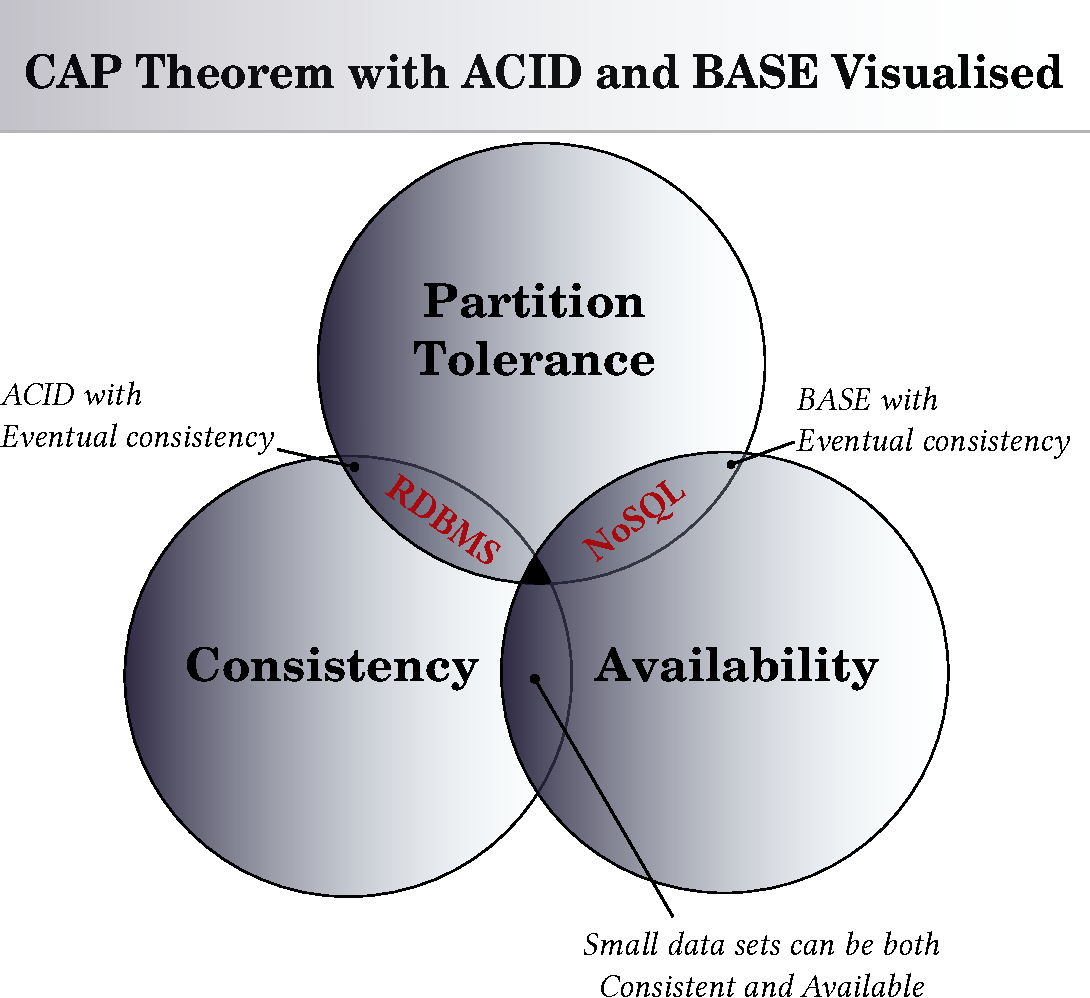
\includegraphics[width=0.8\maxwidth]{../figures/cap-nist.pdf}
        \caption{CAP theorem with ACID and BASE visualized\label{fig:cap}}
       \end{center}
    \end{figure}
\end{description}

\subsection{NoSQL Models}

